\section{Realisierung}
Aus den Dimensionierungen im letzten Kapitel ist nun ein Balun realisiert worden. Zuerst haben wir eine Stufe des Guanella-Baluns gewickelt. Mit einem Impedanzmessgerät konnten wir anschliessend überprüfen, ob Gleichtaktströme bei der gewünschten Arbeitsfrequenz unterdrückt werden. Abbildung \ref{fig:mess_real} zeigt den Aufbau einer solchen Impedanzmessung.
\begin{figure}[H]
	\centering
	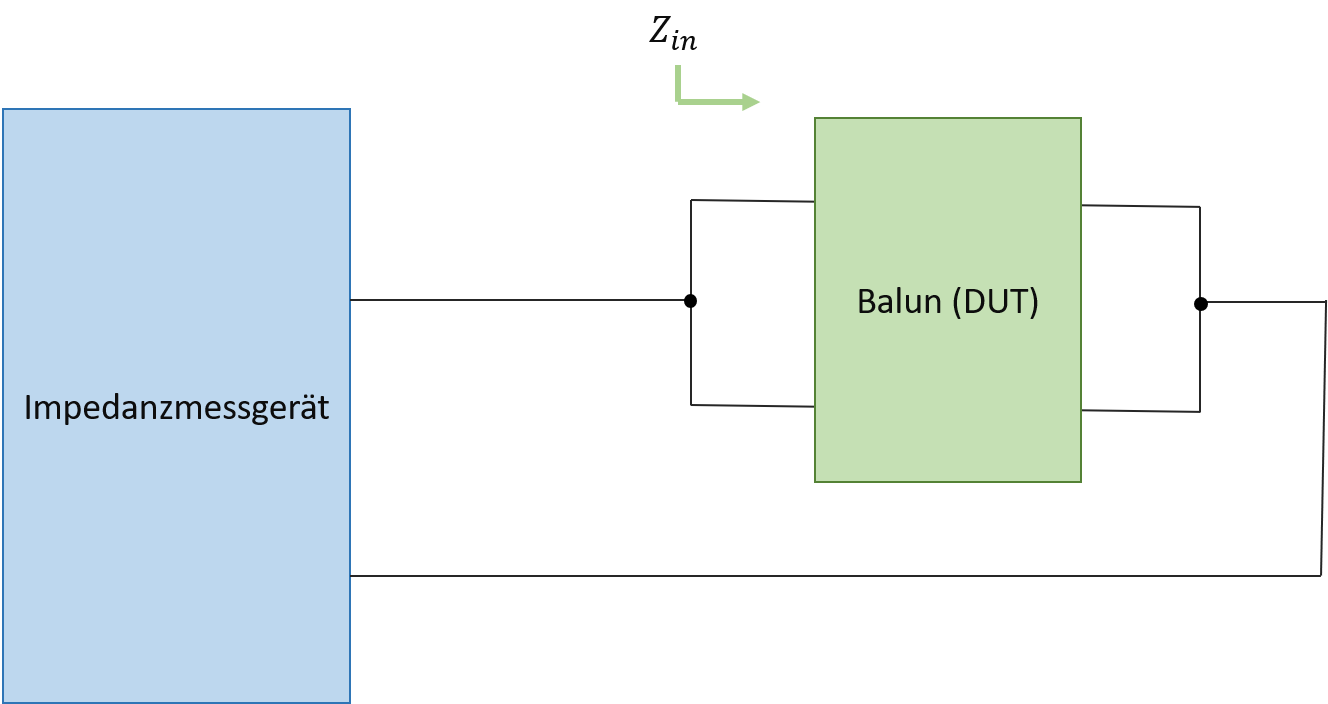
\includegraphics[width=0.7\linewidth]{Messaufbau_realisierung.png}
	\caption{Messaufbau der Impedanzmessung}\label{fig:mess_real}
\end{figure}

Das Messresultat der ersten Messung ist in folgender Abbildung ersichtlich. Man kann erkennen, dass die Resonanzfrequenz nicht wie dimensioniert bei \SI{20}{MHz}, sondern bei ca. \SI{35}{MHz} liegt. Durch Erhöhung der Windungszahl, konnte die Resonanzfrequenz auf \SI{20}{MHz} verändert werden.
\begin{figure}[H]
	\centering
	\includegraphics[width=0.7\linewidth]{Impedanz_dimensionierung.PNG}
	\caption{Messung der Impedanz der ersten Guanella-Balun Stufe}\label{fig:imp_dim}
\end{figure}

Während der Messung hat sich herausgestellt, dass schon leichte Manipulationen (unterschiedlicher Anpressdruck) an der Wicklung die Resonanzfrequenz stark (\textpm 50\%) beeinflussen. Um dem entgegenzuwirken, wurden die beiden Stufen des Baluns mit einer mechanischen Konstruktion fixiert. Dies wird in Abbildung \ref{fig:balun} gezeigt.
\begin{figure}[h!]
	\centering
	\subfloat[Symmetrische Seite]{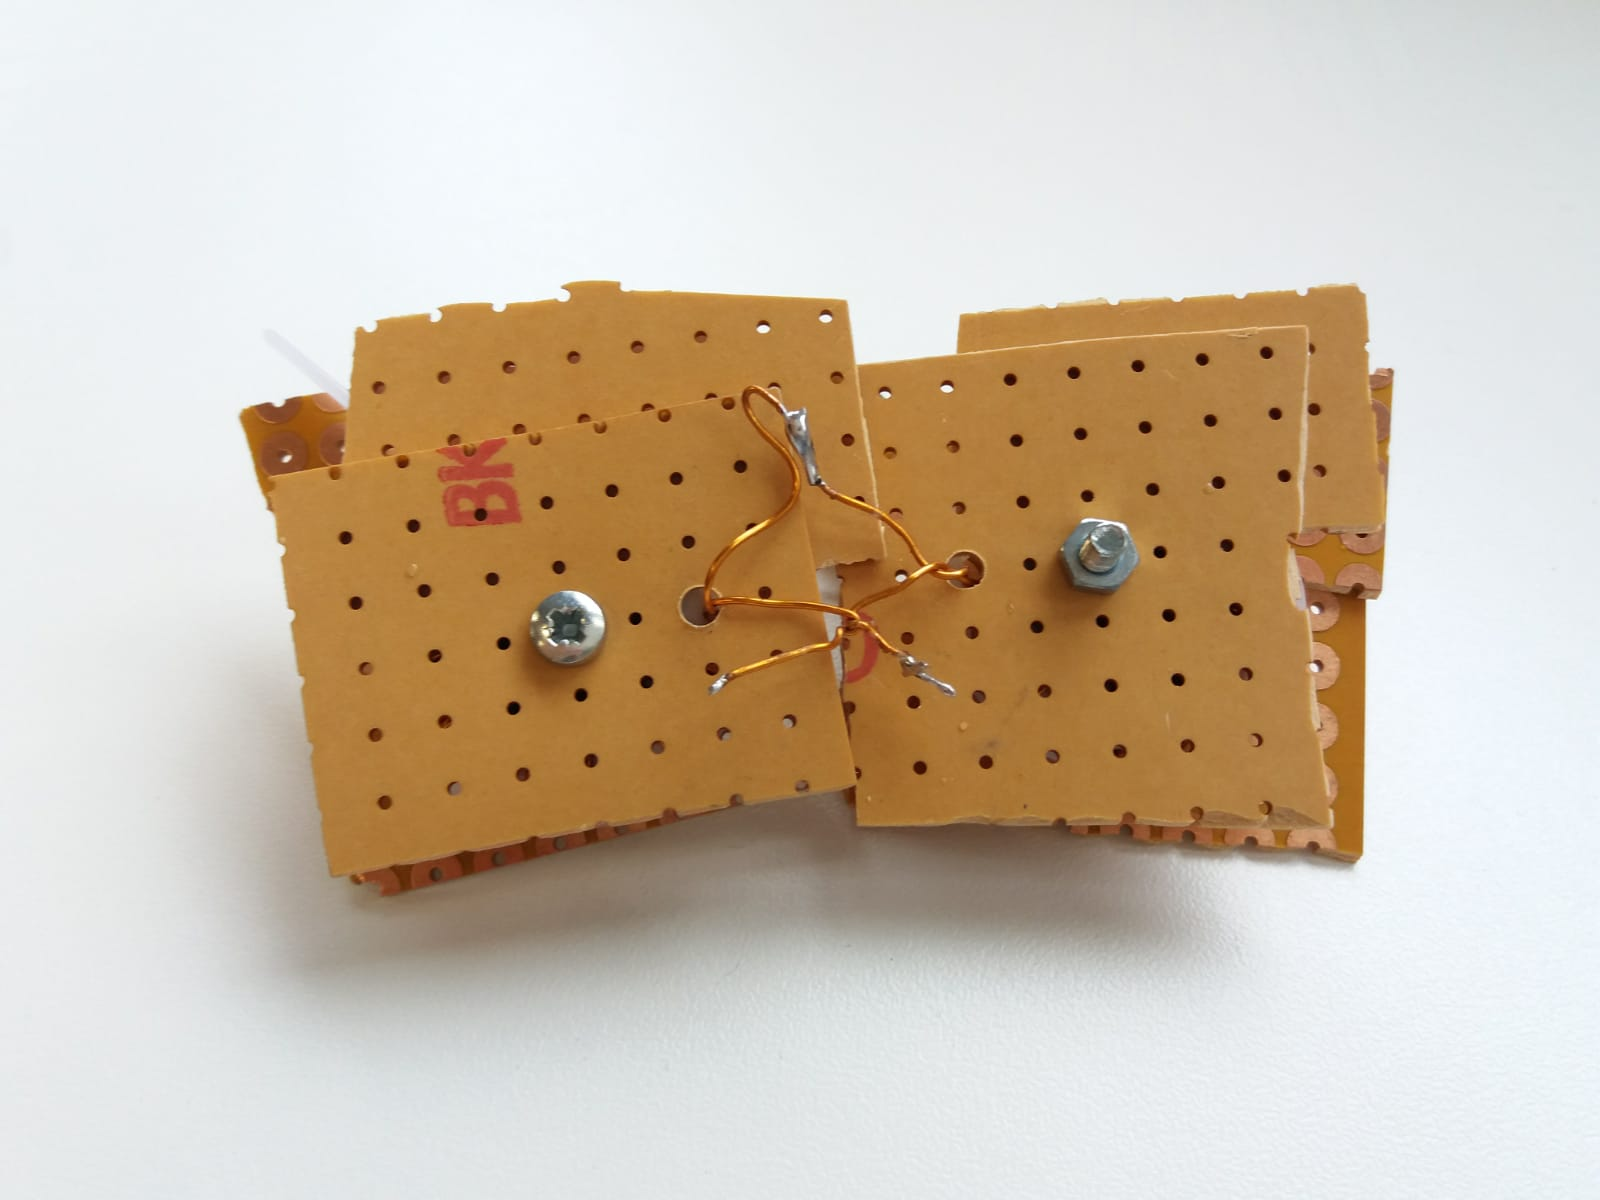
\includegraphics[width=0.5\linewidth]{Balun1.jpg}}\qquad
	\subfloat[Unsymmetrische Seite]{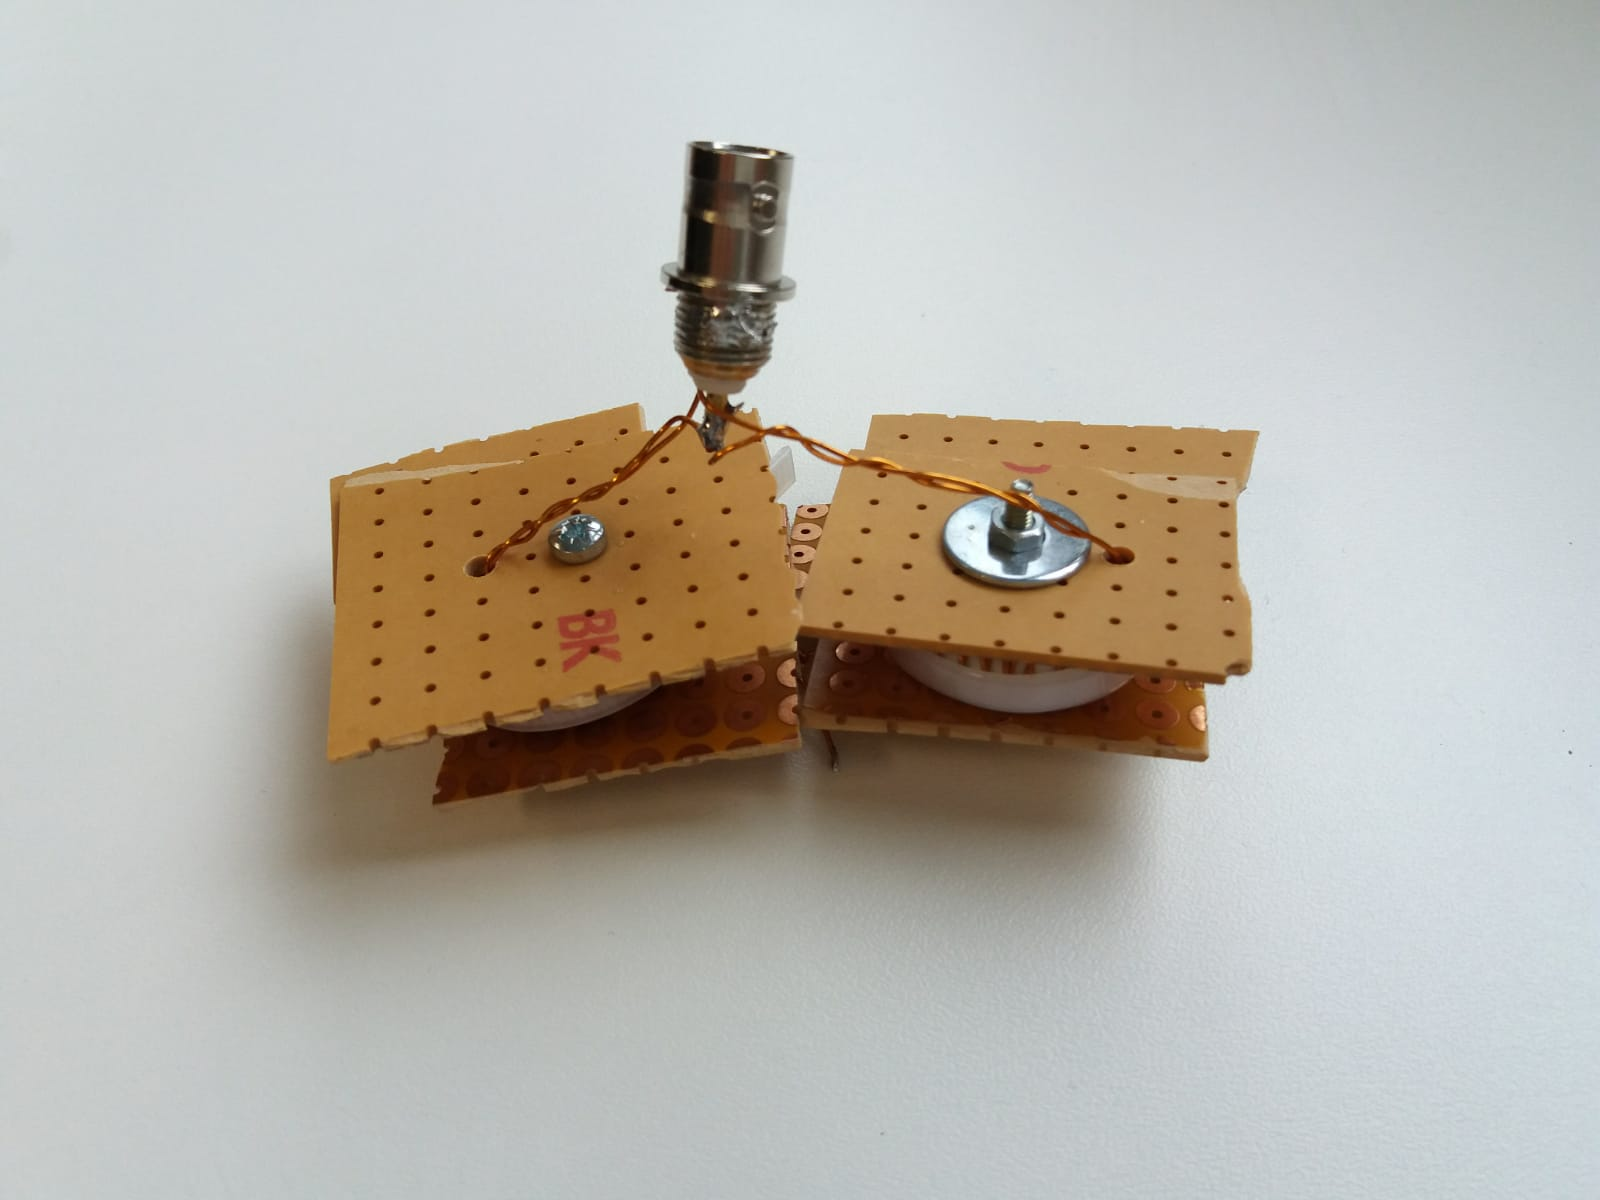
\includegraphics[width=0.5\linewidth]{Balun2.jpg}}\qquad
	\subfloat[Seitenansicht]{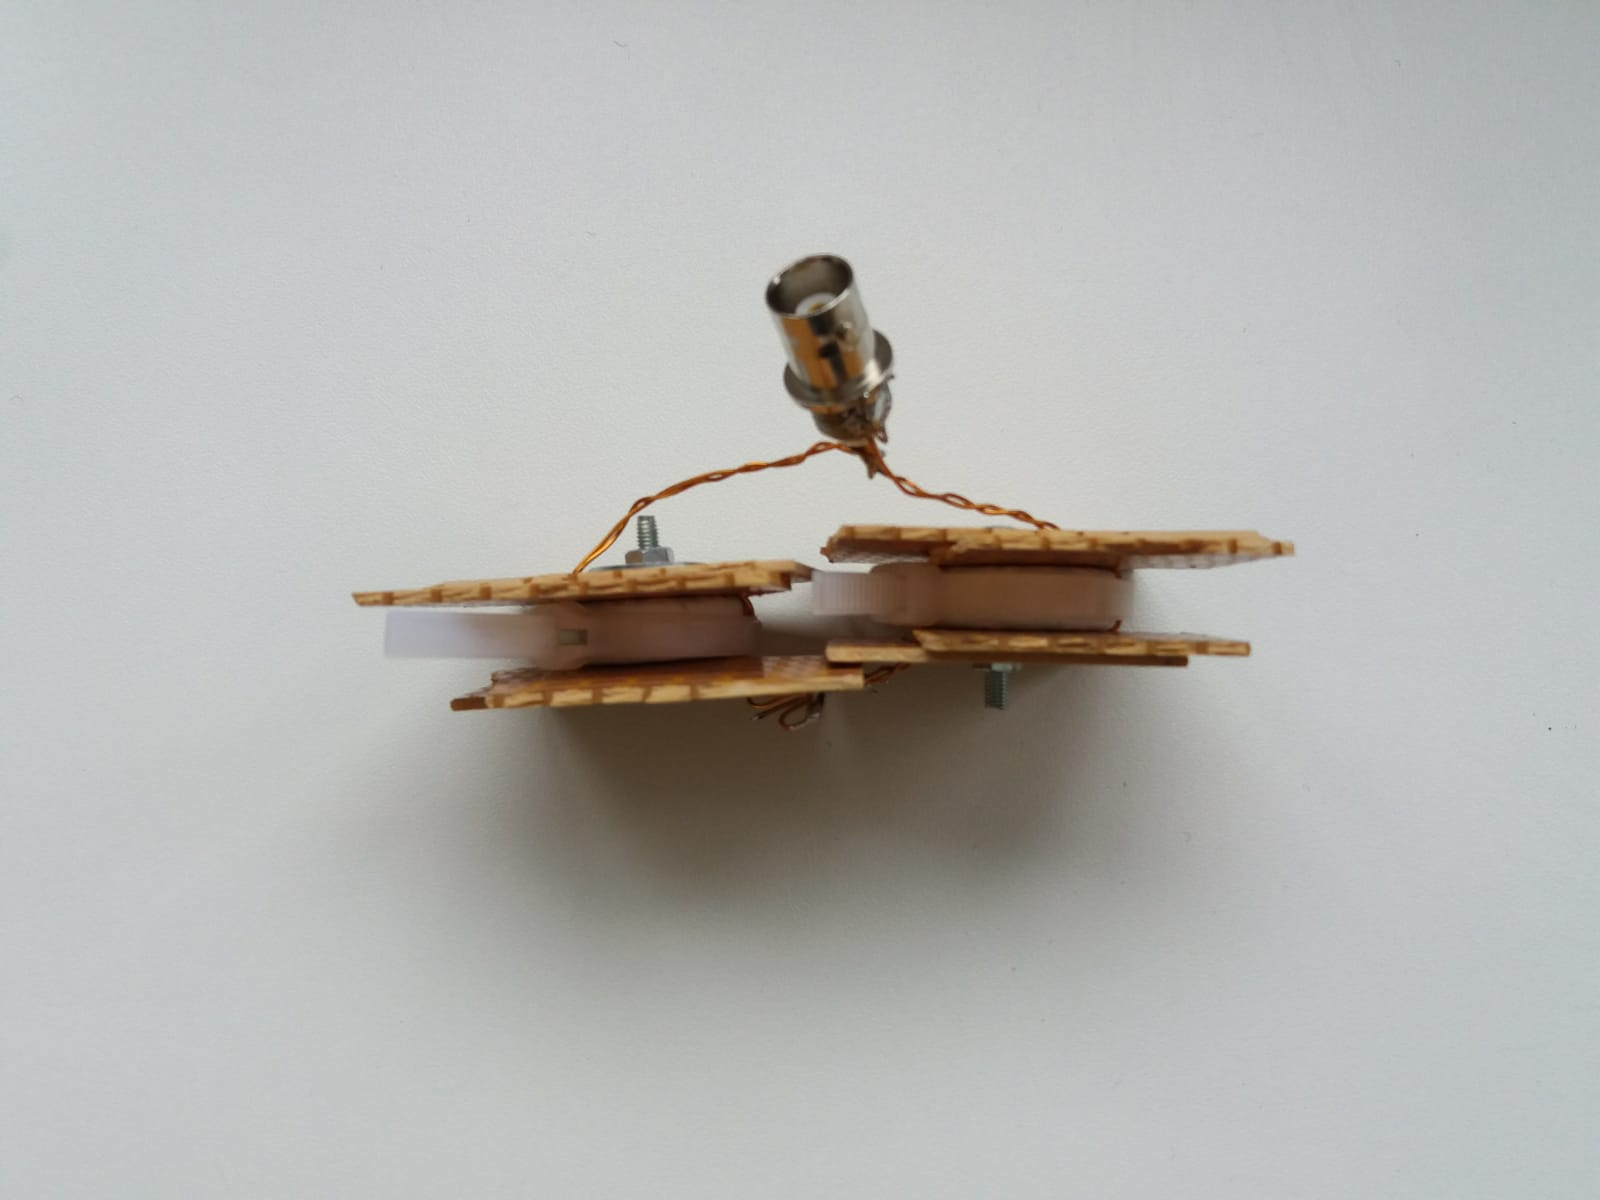
\includegraphics[width=0.5\linewidth]{Balun3.jpg}}
	\caption{Der realisierte Guanella-Balun}
	\label{fig:balun}
\end{figure}
Wie man in den Abbildungen erkennen kann, wurden jeweils zwei Leitungen verdrillt, um die unerwünschten Induktionseffekte zu reduzieren.
